
\section{Systematic uncertainties}
\label{sec:strong:syst}

The sources of systematic uncertainties discussed in Sections \ref{sec:common_syst} and \ref{sec:common_backgrounds} are included in the analysis.
The relative size of these uncertainties after the fit in the \glspl{cr} is shown in Figures \ref{fig:syst_cutandcount} and \ref{fig:syst_multibin},
for the cut-and-count and multi-bin analyses respectively. 
In the figure, the uncertainties are grouped into:
\begin{itemize}
\item Experimental uncertainties, that contain the sum in quadrature of the detector-related uncertainties 
presented in Section \ref{sec:common_syst}. These are considered for both the background and signal \gls{mc} samples.
The ranking of the different sources of uncertainty changes from region to region; in general the dominant ones are \gls{jes} (that has a 
relative impact on the expected background between 4 and 35\% in the different \glspl{sr}), \gls{jer} (0-26\%) and the uncertainties on the 
b-tagging efficiency and mistagging rate (3-24\%).

\item Theoretical uncertainties, which are the sum in quadrature of the modelling systematics discussed in Section \ref{sec:common_backgrounds}.
In this case the dominant uncertainties are the ones on the modelling of the \ttbar background, whose impact ranges between 5 and 76\%).

\item \gls{mc} statistical uncertainty.

\item Statistical uncertainty in the \glspl{cr}, that is reflected in the uncertainty on the \ttbar scale factor and takes values between 10 and 30\%.

\end{itemize}

The total uncertainty (black line in Figure \ref{fig:syst}) takes into account correlation effects across the different systematic sources, 
and therefore is not the sum in quadrature of the individual components. 

\begin{figure}[ht]
	\centering
	\subfigure[]{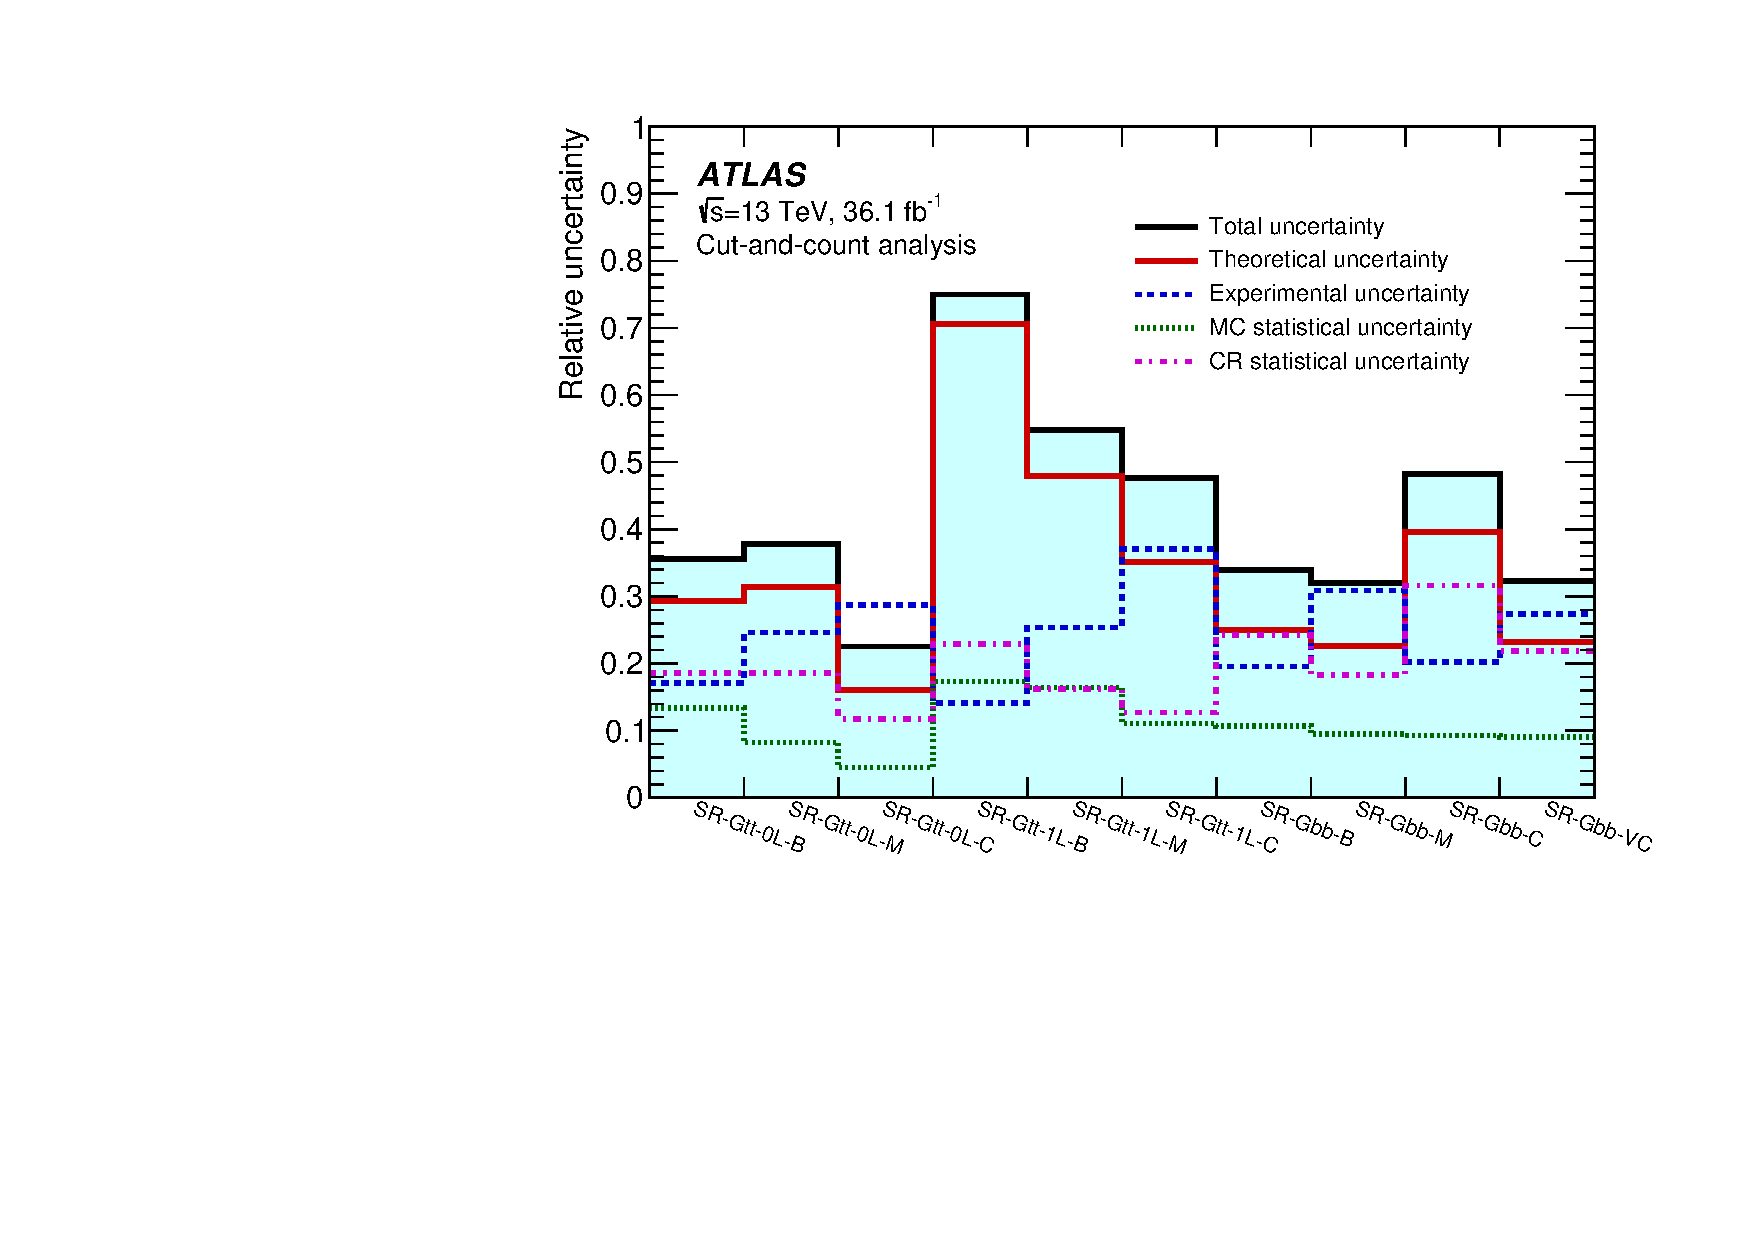
\includegraphics[width=0.85\textwidth]{figures/strong_prod/paper/Cut_and_Count.pdf}\label{fig:syst_cutandcount}}\\
	\subfigure[]{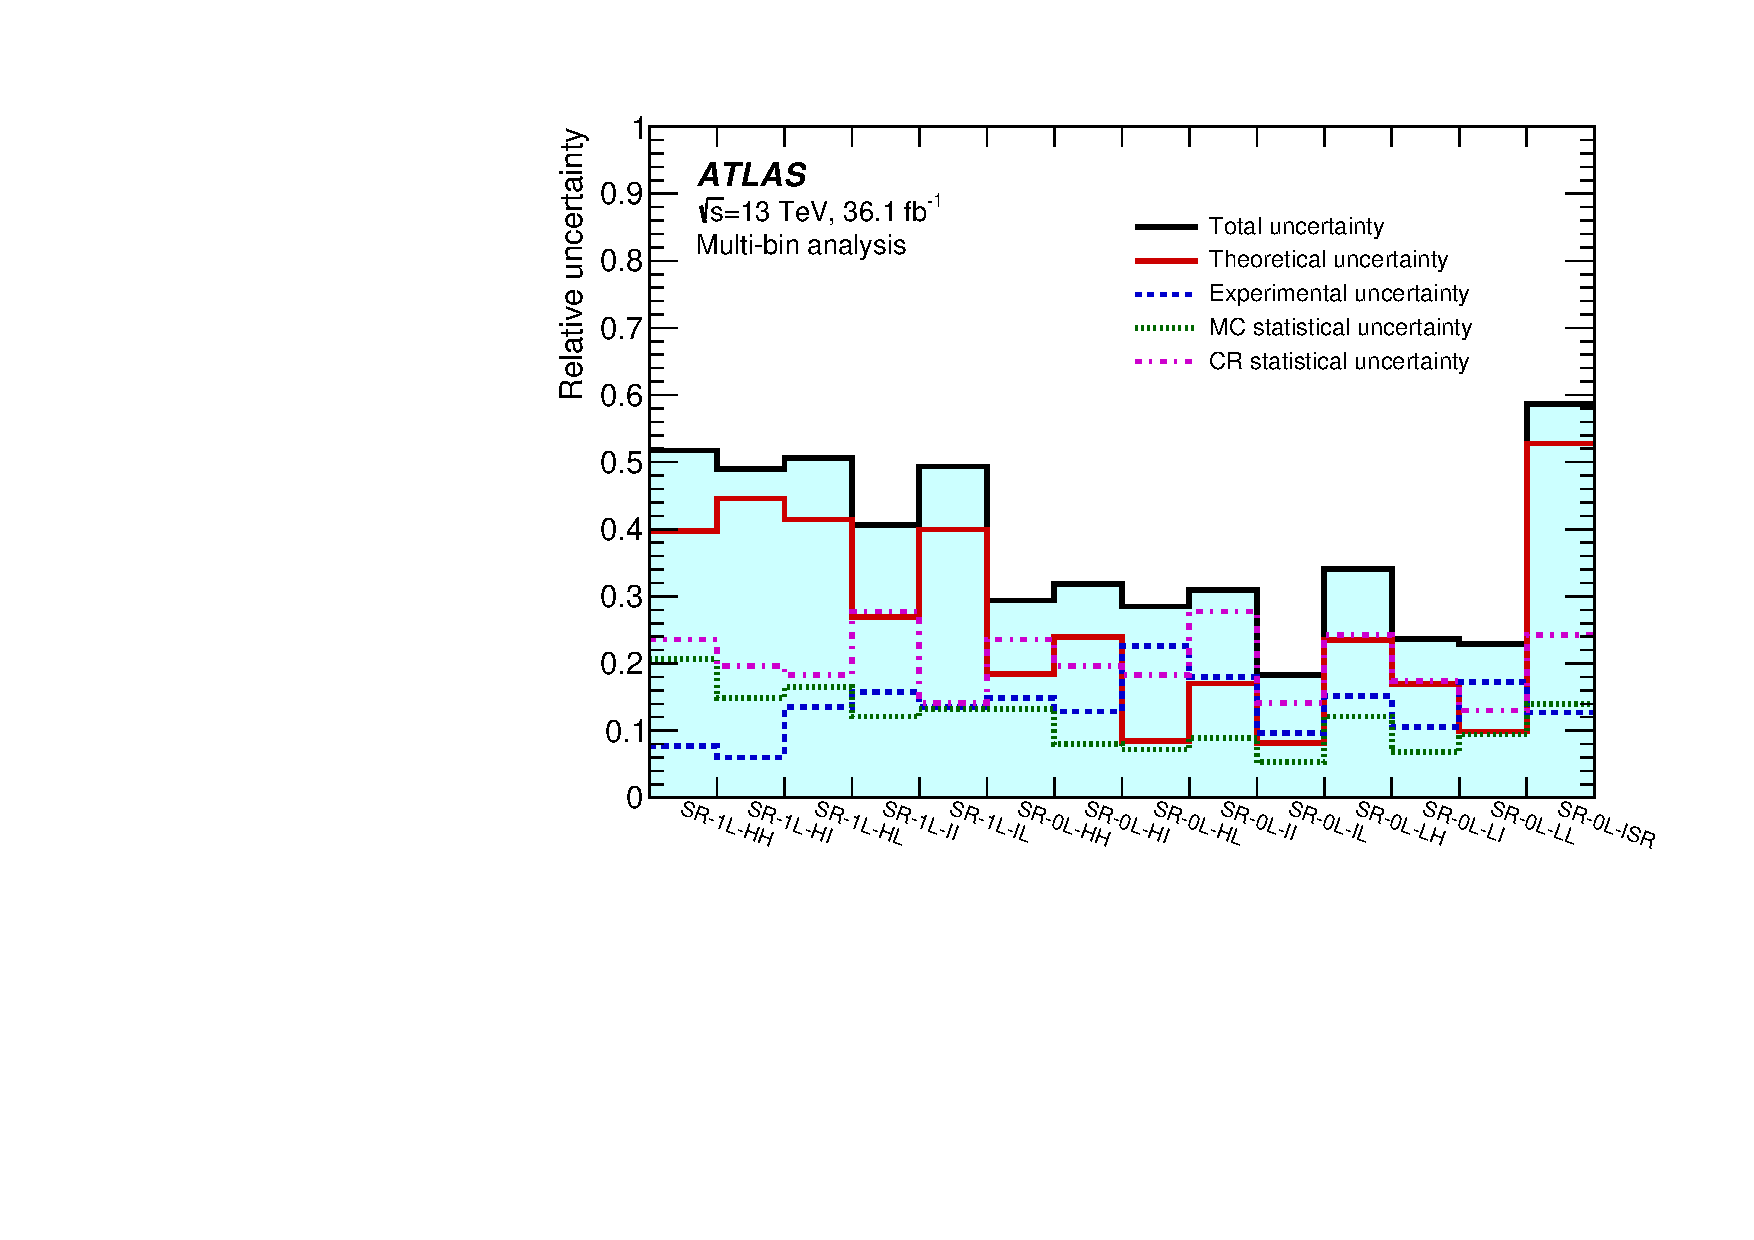
\includegraphics[width=0.85\textwidth]{figures/strong_prod/paper/Multi_bin.pdf}\label{fig:syst_multibin}}\\
	\caption{Relative systematic uncertainty in the background estimate for the \subref{fig:syst_cutandcount} cut-and-count and \subref{fig:syst_multibin} multi-bin analyses. The individual uncertainties can be correlated, such that the total background uncertainty is not necessarily their sum in quadrature.
	} 
	\label{fig:syst}
\end{figure}

\section{Results}

\begin{figure}[ht]
	\centering
	\subfigure[]{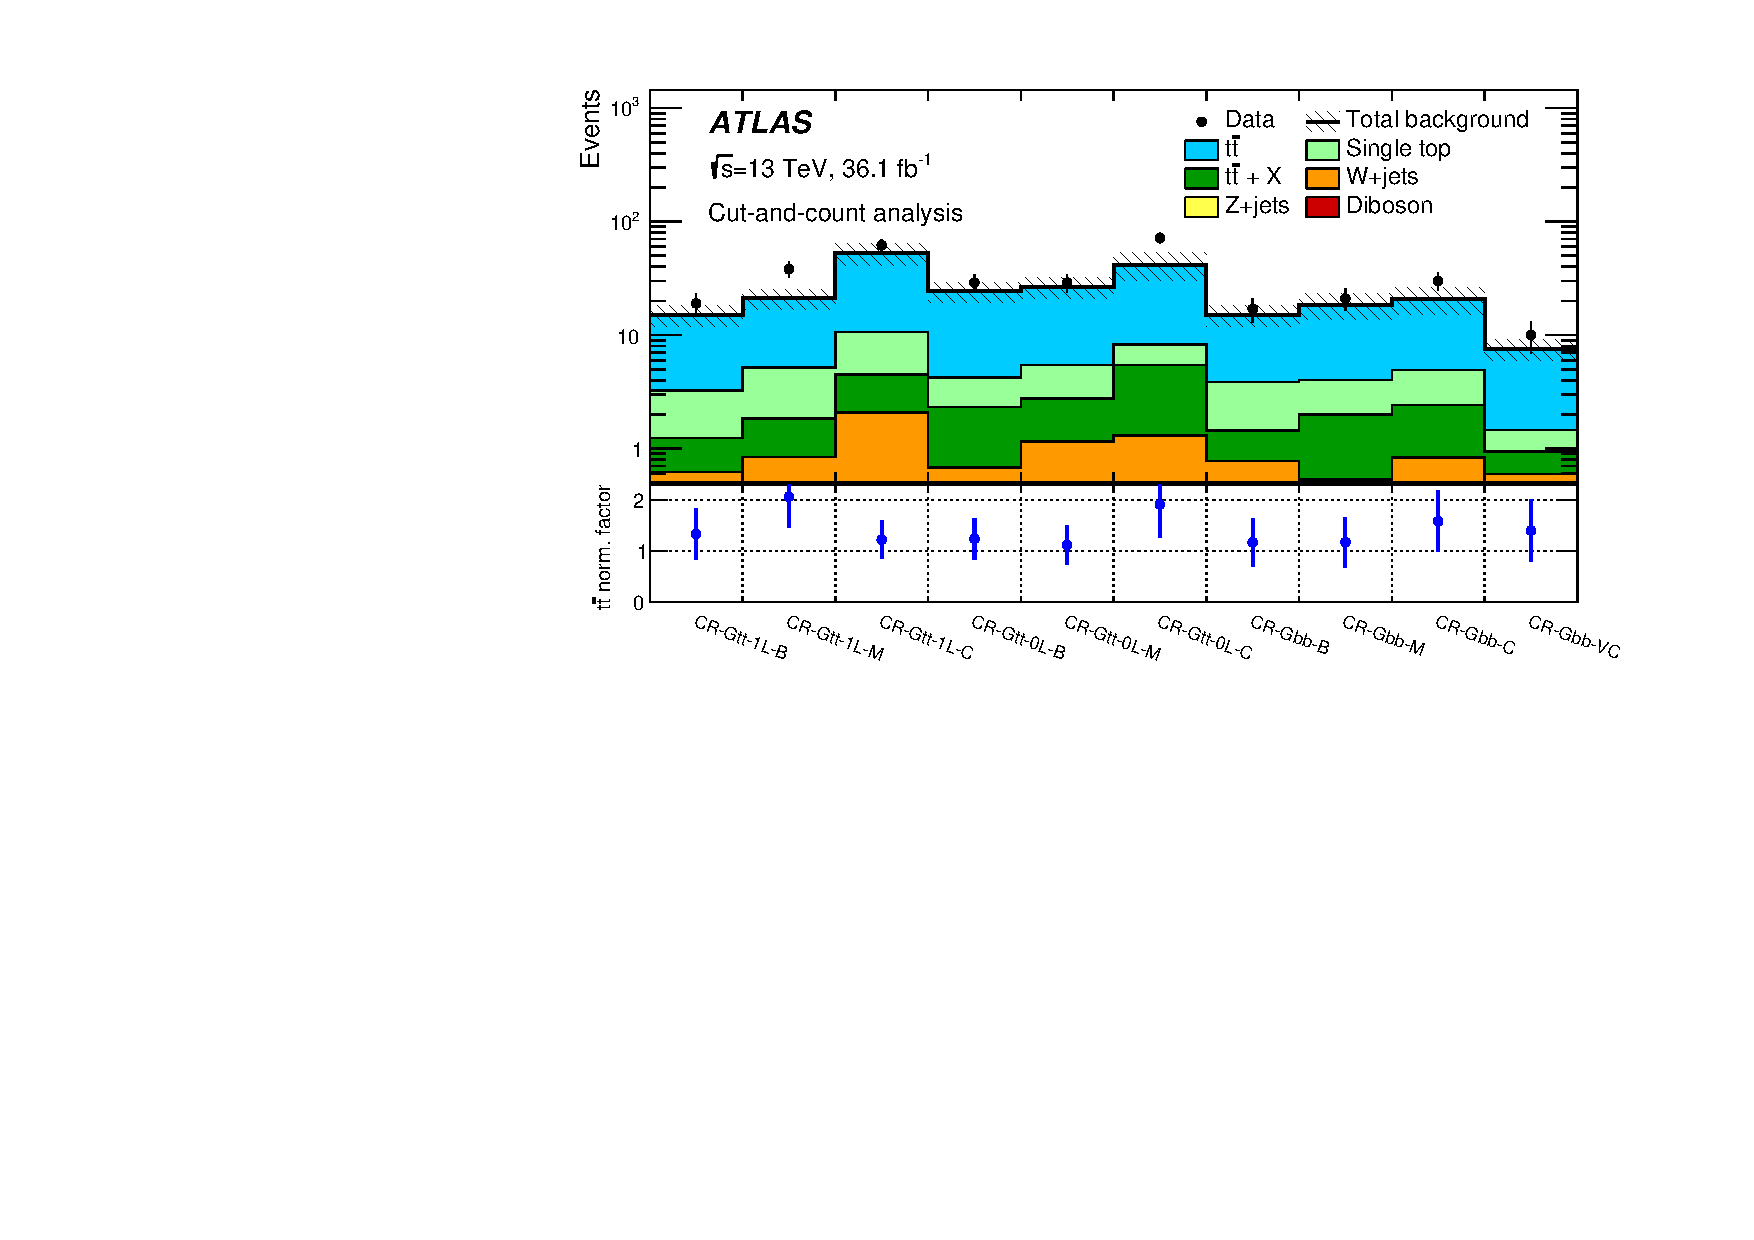
\includegraphics[width=0.9\textwidth]{figures/strong_prod/paper/pulls/histpull_pulls_in_CRs_17_06_23_singlebin.pdf}\label{fig:pullCR_discovery}}
	\subfigure[]{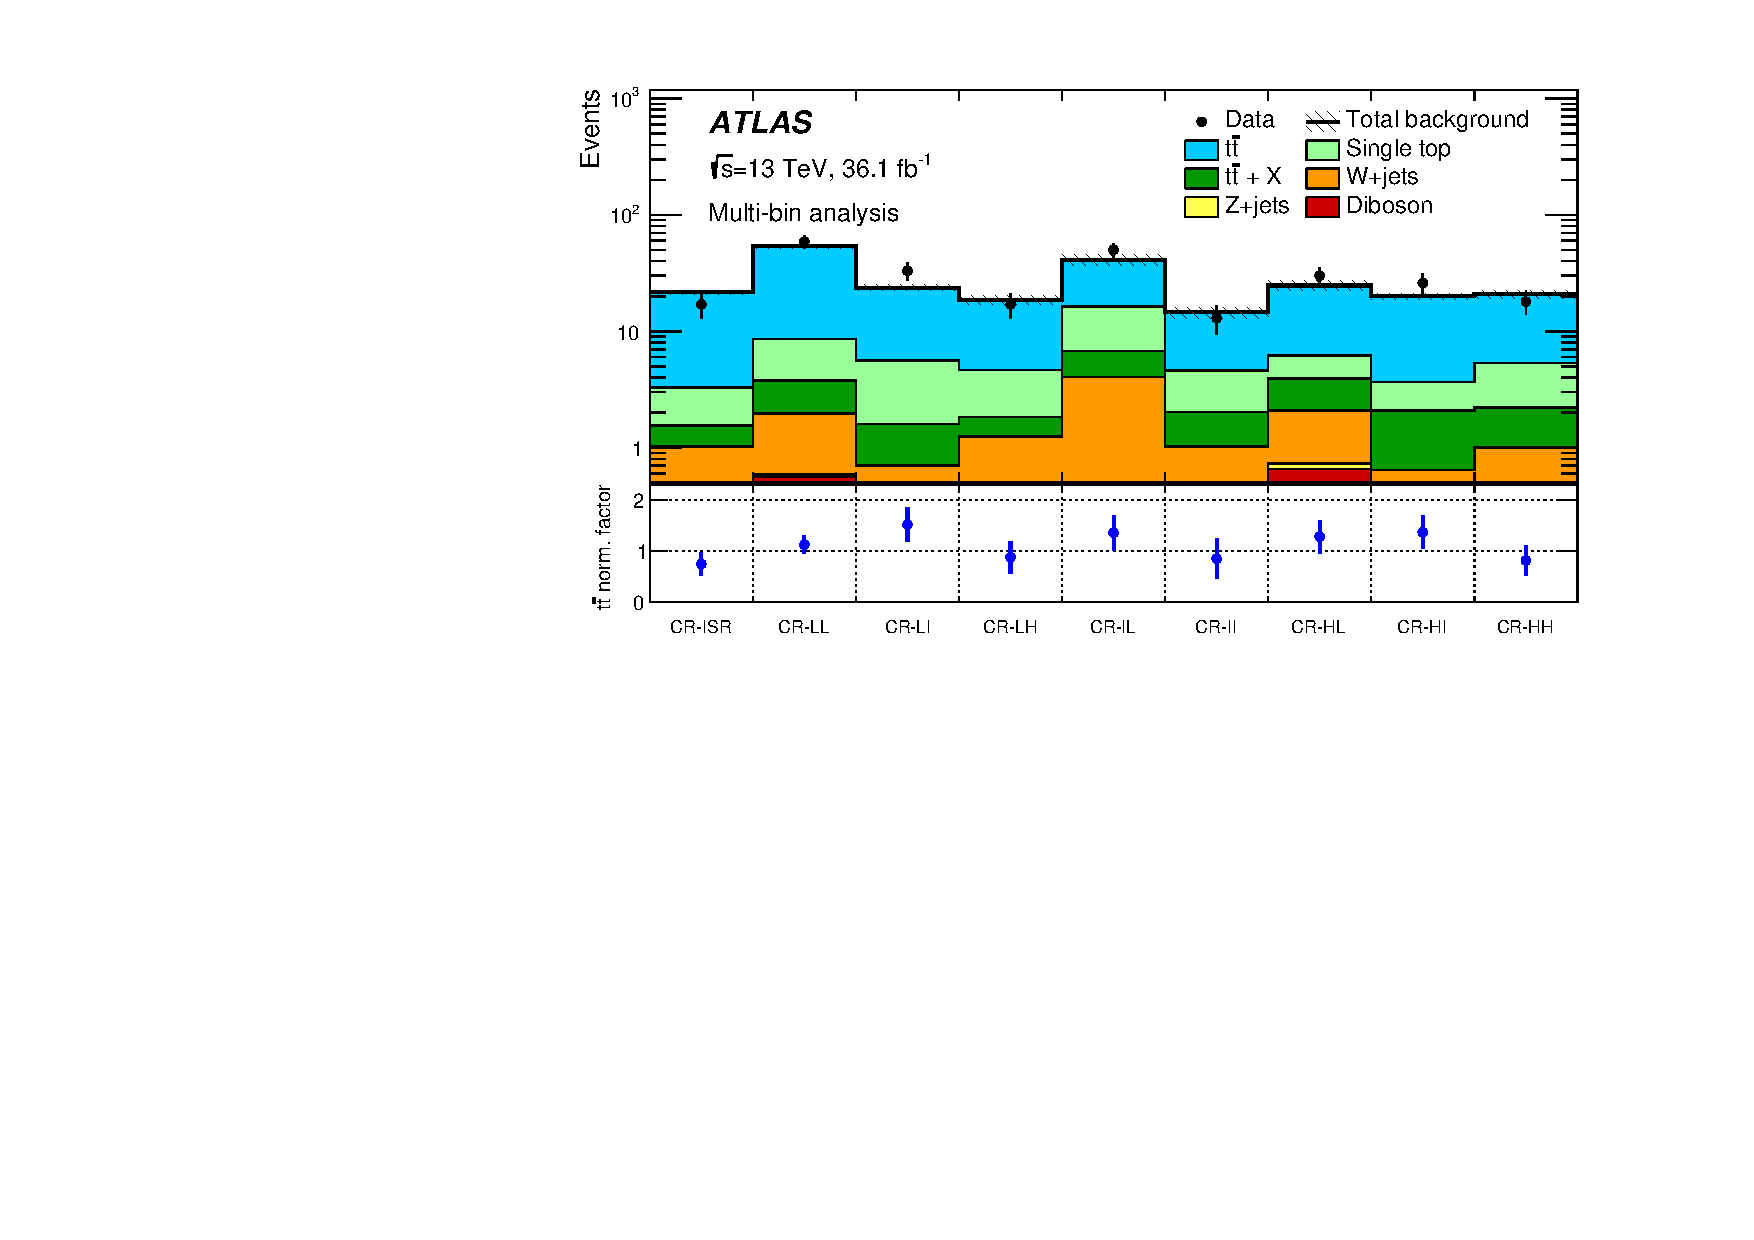
\includegraphics[width=0.9\textwidth]{figures/strong_prod/paper/pulls/histpull_pulls_in_CRs_multichannel_17_06_23.pdf}\label{fig:pullCR_exclusion}}
	\caption{Pre-fit event yield in control regions and related \ttbar
          normalization factors after the background-only fit for
          \subref{fig:pullCR_discovery} 
		the cut-and-count and \subref{fig:pullCR_exclusion} the multi-bin analyses. The upper panel shows 
		the observed number of events and the predicted background yield before the fit.
		The background category \ttbar+X includes \ttbar+W/Z, \ttbar+H and \ttbar\ttbar events. All of these
                regions require at least one signal lepton, for which the
                multijet background is negligible. All uncertainties describes in Section \ref{sec:strong:syst} are included in the uncertainty band.
		The \ttbar normalisation is obtained from the fit
                and is displayed in the bottom panel. 
	} 
	\label{fig:pullCR}
\end{figure}


\begin{figure}[ht]
	\centering
	\subfigure[]{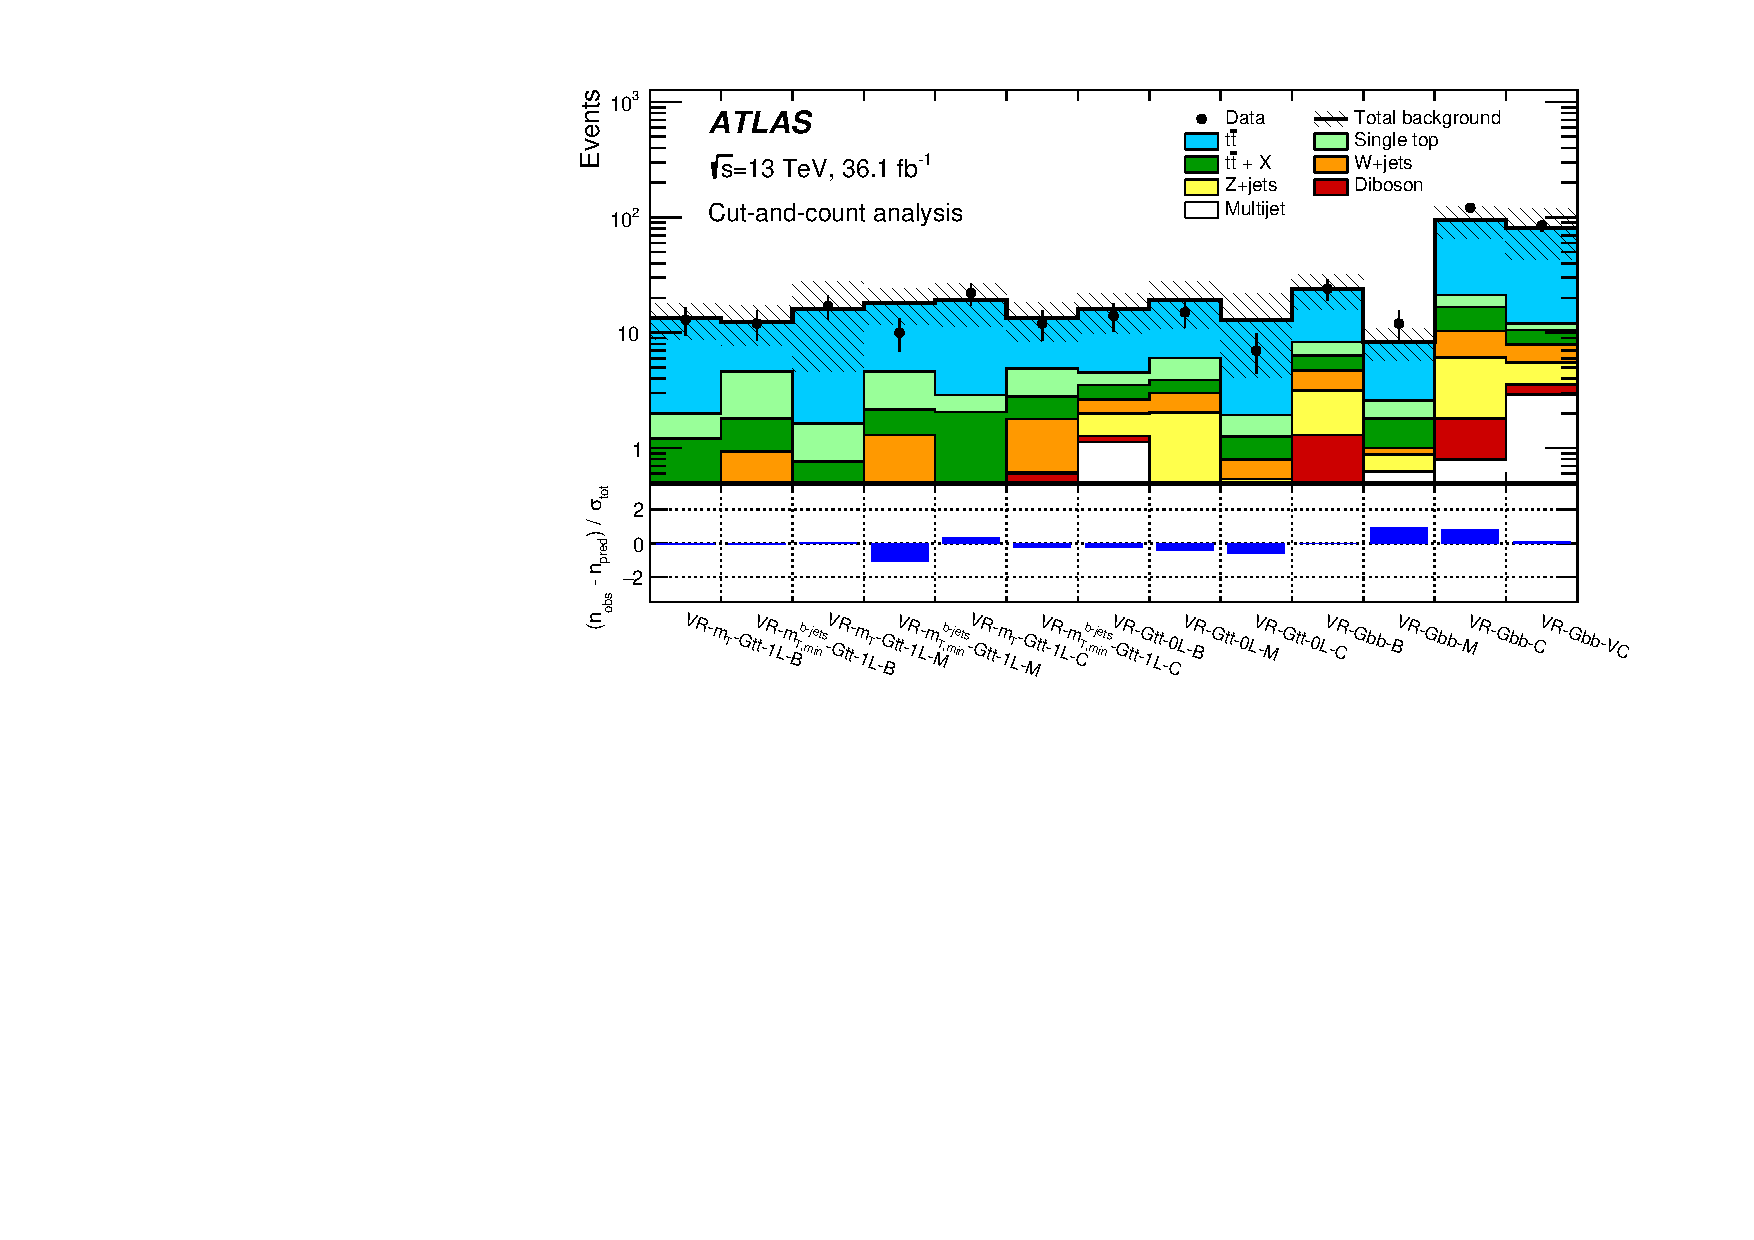
\includegraphics[width=0.9\textwidth]{figures/strong_prod/paper/pulls/histpull_pulls_in_VRs_17_06_23_singlebin.pdf}\label{fig:pullVR_discovery}}\\
	\subfigure[]{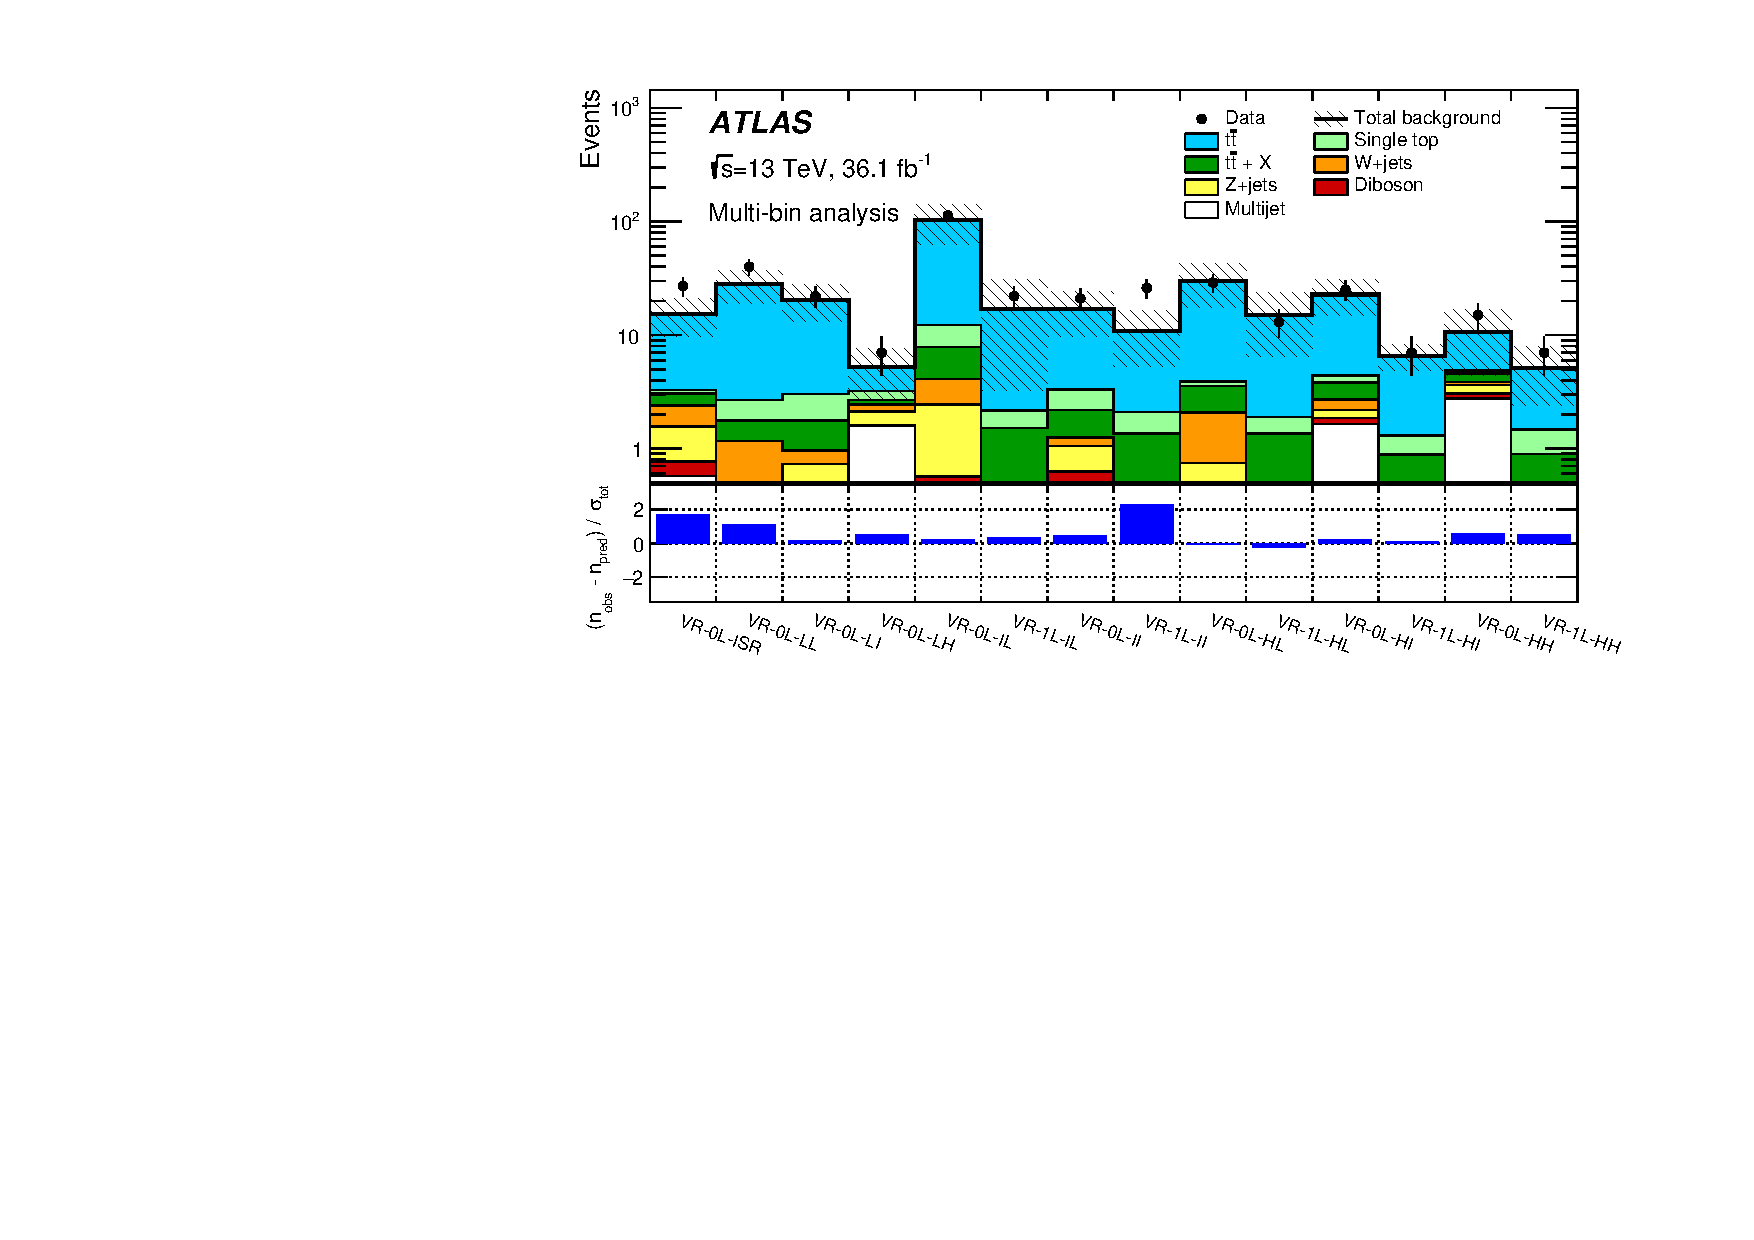
\includegraphics[width=0.9\textwidth]{figures/strong_prod/paper/pulls/histpull_pulls_in_VRs_multichannel_17_06_23.pdf}\label{fig:pullVR_exclusion}}\\
	\caption{Results of the background-only fit extrapolated to the VRs of \subref{fig:pullVR_discovery} the cut-and-count and \subref{fig:pullVR_exclusion}
		the multi-bin analyses. The \ttbar normalisation 
		is obtained from the fit to the CRs shown in Figure~\ref{fig:pullCR}. The upper panel shows 
		the observed number of events and the predicted background yield.
		All uncertainties  defined in Section~\ref{sec:syst} are included in the 
		uncertainty band. The background category \ttbar+X includes \ttbar+W/Z, 
		\ttbar+H and \ttbar\ttbar events. The lower panel shows the pulls in 
		each VR. 
	} 
	\label{fig:pullVR}
\end{figure}


\begin{figure}[ht]
	\centering
	\subfigure[]{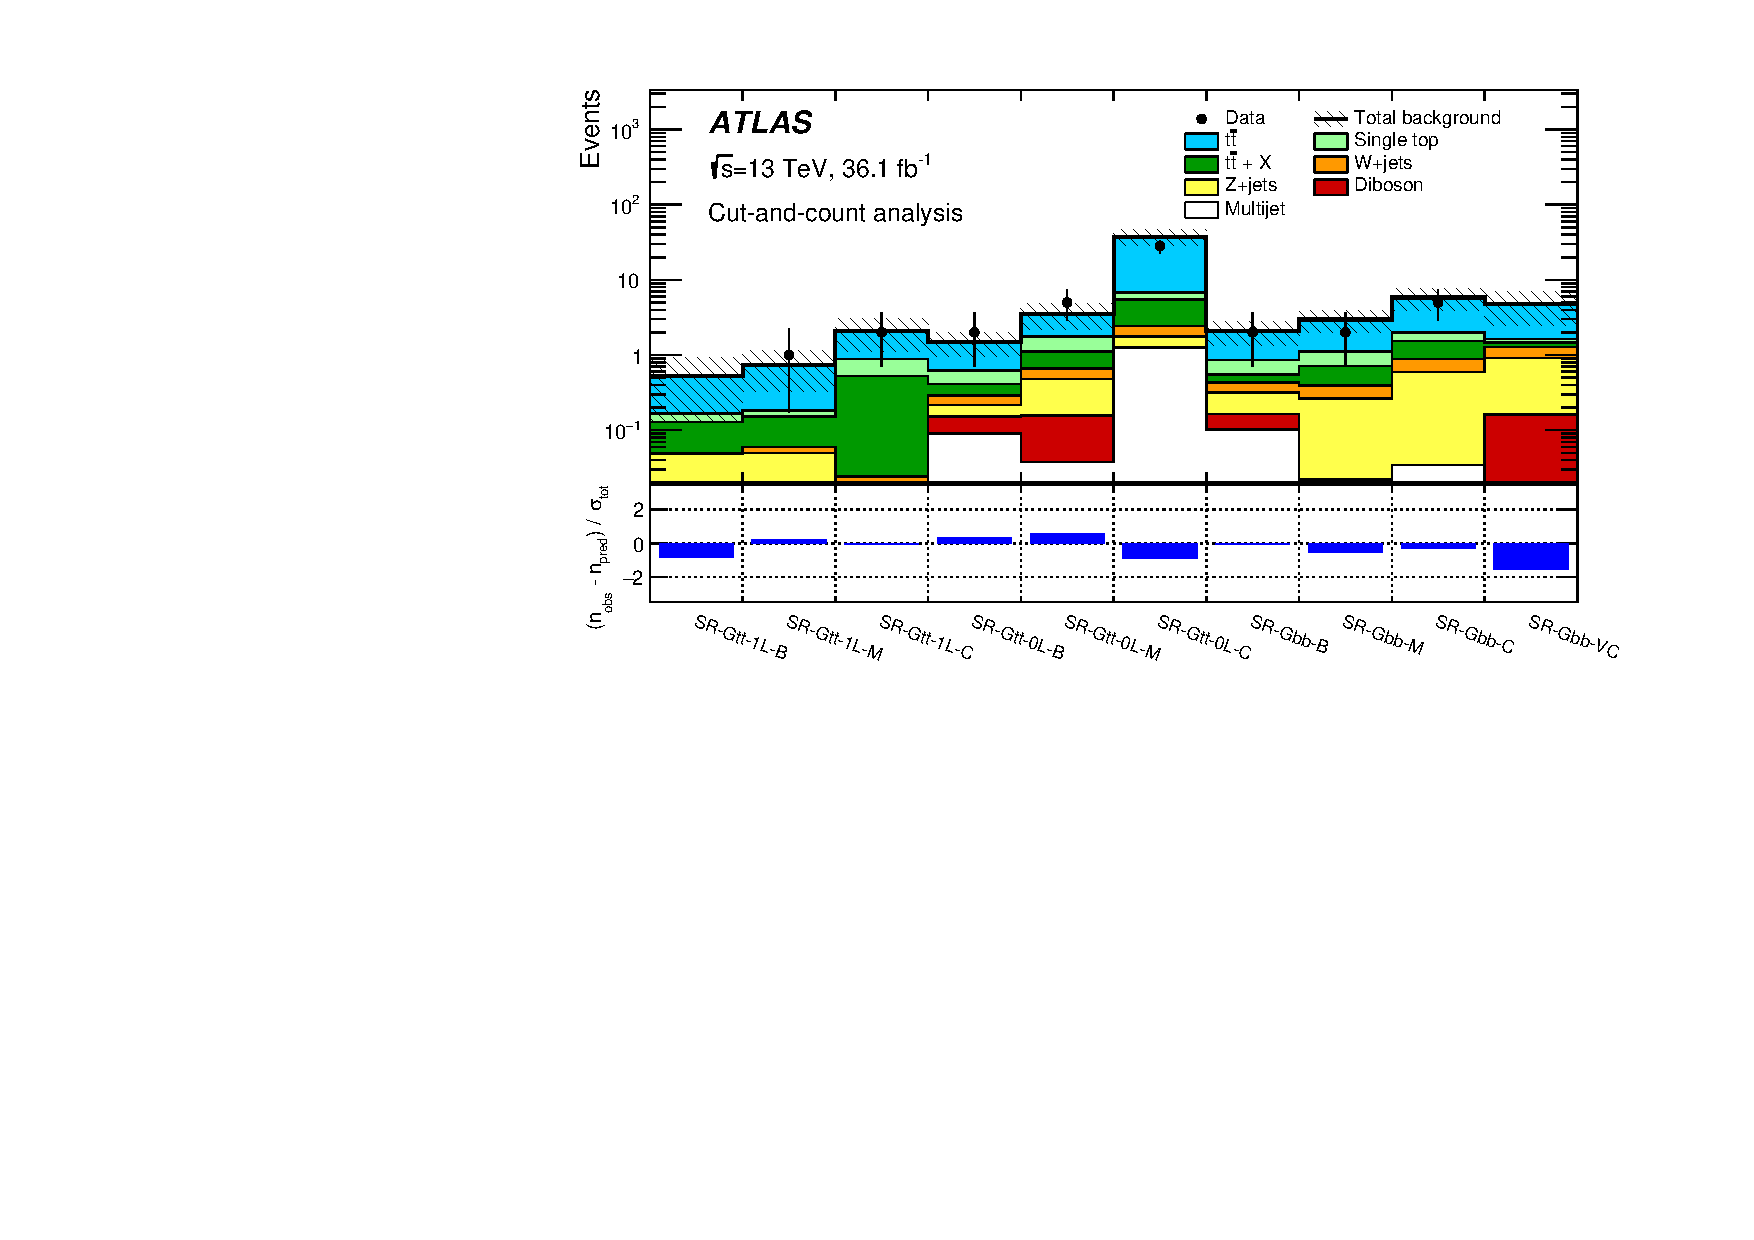
\includegraphics[width=0.9\textwidth]{figures/strong_prod/paper/pulls/histpull_pulls_in_SRs_17_06_23_singlebin.pdf}\label{fig:pullSR_discovery}}\\
	\subfigure[]{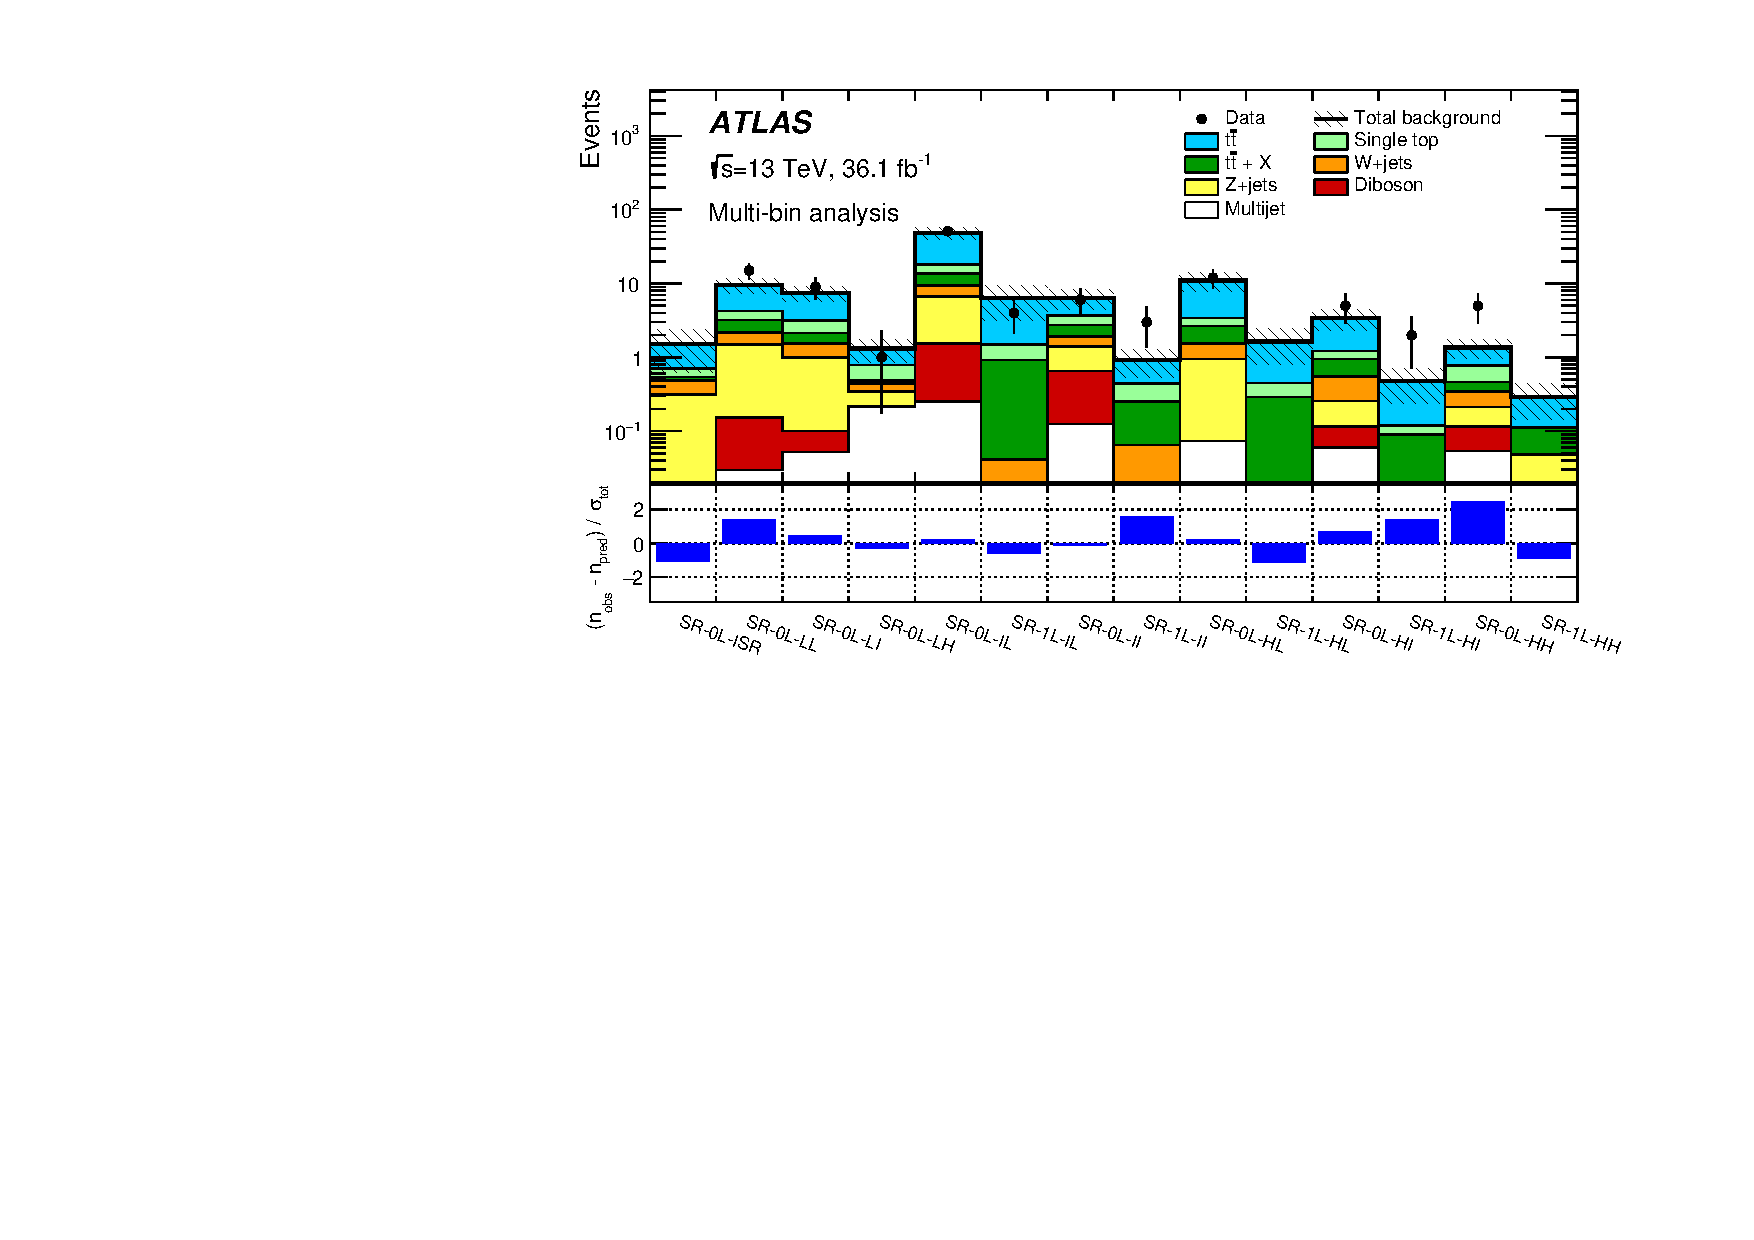
\includegraphics[width=0.9\textwidth]{figures/strong_prod/paper/pulls/histpull_pulls_in_SRs_multichannel_17_06_23.pdf}\label{fig:pullSR_exclusion}}\\
	\caption{Results of the background-only fit extrapolated to the SRs for \subref{fig:pullSR_discovery}
	the cut-and-count and \subref{fig:pullSR_exclusion} the multi-bin analyses. The data in the  SRs are 
	not included in the fit.  The upper panel shows the observed number of events and the predicted background 
	yield. All uncertainties  defined in Section~\ref{sec:syst} are included in the uncertainty band. The background 
	category $\ttbar+X$ includes $\ttbar W/Z$, $\ttbar H$ and $\ttbar \ttbar$ events. The lower panel shows the 
	pulls in each SR.} 
	\label{fig:pullSR}
\end{figure}

%\clearpage 
\FloatBarrier

\section{Interpretation}

\subsection{Model-independent limits}

\begin{table}[t]
        \centering
        \small
        \begin{tabular*}{0.6\textwidth}{@{\extracolsep{\fill}}lcccc}
                \noalign{\smallskip}\toprule\noalign{\smallskip}
                Signal channel         & $p_0$ (Z)            & $\sigma^{95}_\mathrm{vis}$ [fb]  &  $S_{\textrm obs}^{95}$  & $S_{\textrm exp}^{95}$   \\
                \noalign{\smallskip}\midrule \noalign{\smallskip}
                SR-Gtt-1L-B & $ 0.50~(0.00) $ &  $0.08$ &  $3.0$ & $ { 3.0 }^{ +1.0 }_{ -0.0 }$ \\[1mm]
                SR-Gtt-1L-M & $ 0.34~(0.42)$ &  $0.11$ &  $3.9$ & $ { 3.6 }^{ +1.1 }_{ -0.4 }$ \\[1mm]
                SR-Gtt-1L-C & $ 0.50~(0.00)$ &  $0.13$ &  $4.8$ & $ { 4.7 }^{ +1.8 }_{ -0.9 }$ \\[1mm]
                \noalign{\smallskip}\midrule \noalign{\smallskip}
                SR-Gtt-0L-B & $ 0.32~(0.48)$ & $0.13$ &  $4.8$ & $ { 4.1 }^{ +1.7 }_{ -0.6 }$  \\[1mm]
                SR-Gtt-0L-M & $ 0.25~(0.69)$ &  $0.21$ &  $7.5$ & $ { 6.0 }^{ +2.3 }_{ -1.4 }$ \\[1mm]
                SR-Gtt-0L-C & $ 0.50~(0.00)$ &  $0.39$ &  $14.0$ & $ { 17.8 }^{ +6.6 }_{ -4.5 }$ \\[1mm] %%to be updated
                \noalign{\smallskip}\midrule\noalign{\smallskip}
                SR-Gbb-B & $ 0.50~(0.00) $ &  $0.13$ &  $4.6$ & $ { 4.6 }^{ +1.7 }_{ -1.0 }$  \\[1mm]
                SR-Gbb-M & $ 0.50~(0.00) $ & $0.12$ &  $4.4$ & $ { 5.0 }^{ +1.9 }_{ -1.1 }$ \\[1mm]
                SR-Gbb-C & $ 0.50~(0.00) $ &  $0.18$ &  $6.6$ & $ { 6.9 }^{ +2.7 }_{ -1.8 }$ \\[1mm]
                SR-Gbb-VC & $ 0.50~(0.00) $ &  $0.08$ &  $3.0$ & $ { 4.6 }^{ +2.0 }_{ -1.3 }$\\
                \noalign{\smallskip}\midrule\noalign{\smallskip}
        \end{tabular*}
                \caption{The $p_0$-values and $Z$ (the number of equivalent Gaussian standard deviations), 
        	the 95$\%$ CL upper limits on the visible cross-section
                ($\sigma^{95}_\mathrm{vis}$),
                and the observed and
                expected 95$\%$ CL upper limits on the number of BSM events ($S_{\textrm
                obs}^{95}$ and $S_{\textrm exp}^{95}$). The maximum
              allowed $p_0$-value
              is truncated at 0.5.}
        \label{mod-ind-lim}
\end{table}

\subsection{Model-dependent limits}

\begin{figure}[ht]
	\centering 
	\subfigure[]{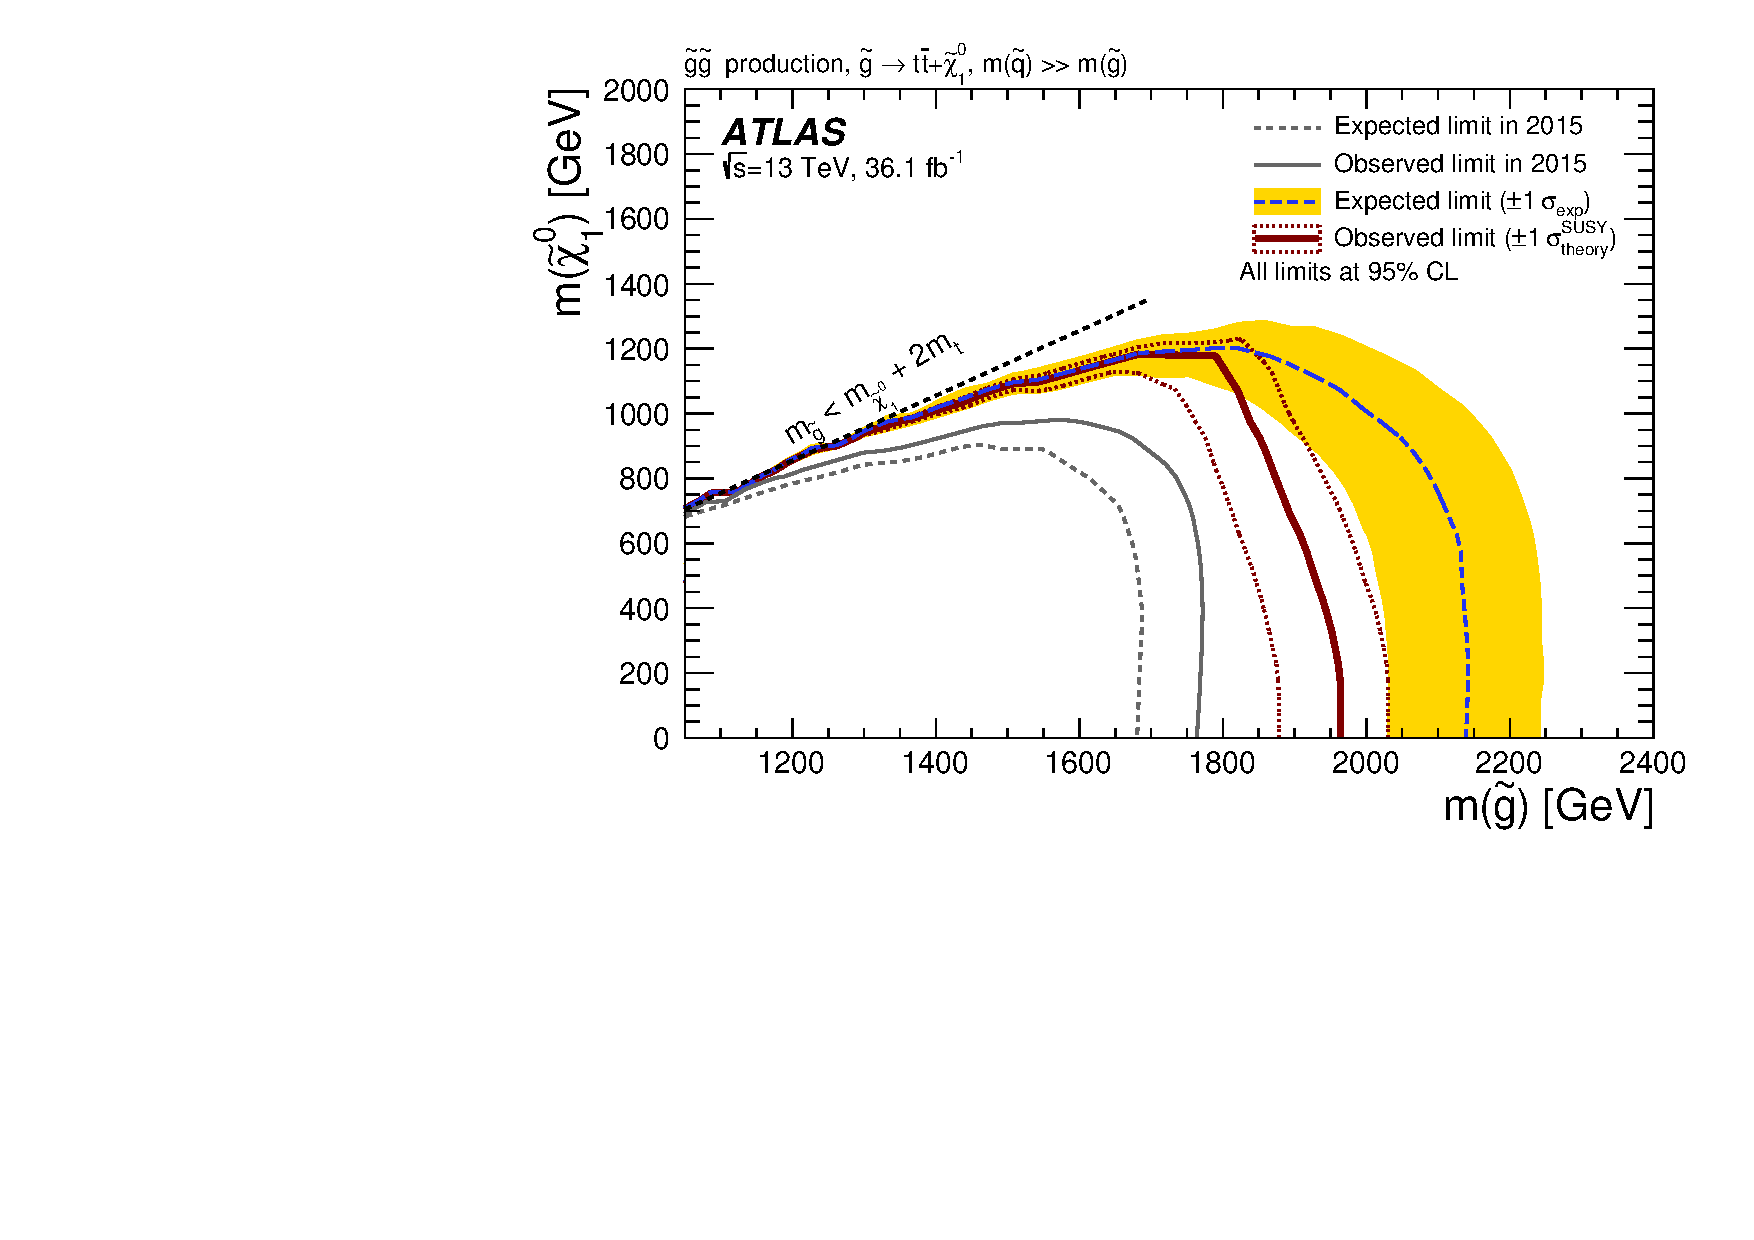
\includegraphics[width=0.75\textwidth]{figures/strong_prod/paper/limits/Limits_Gtt.pdf}\label{fig:limits_Gtt}}
	\subfigure[]{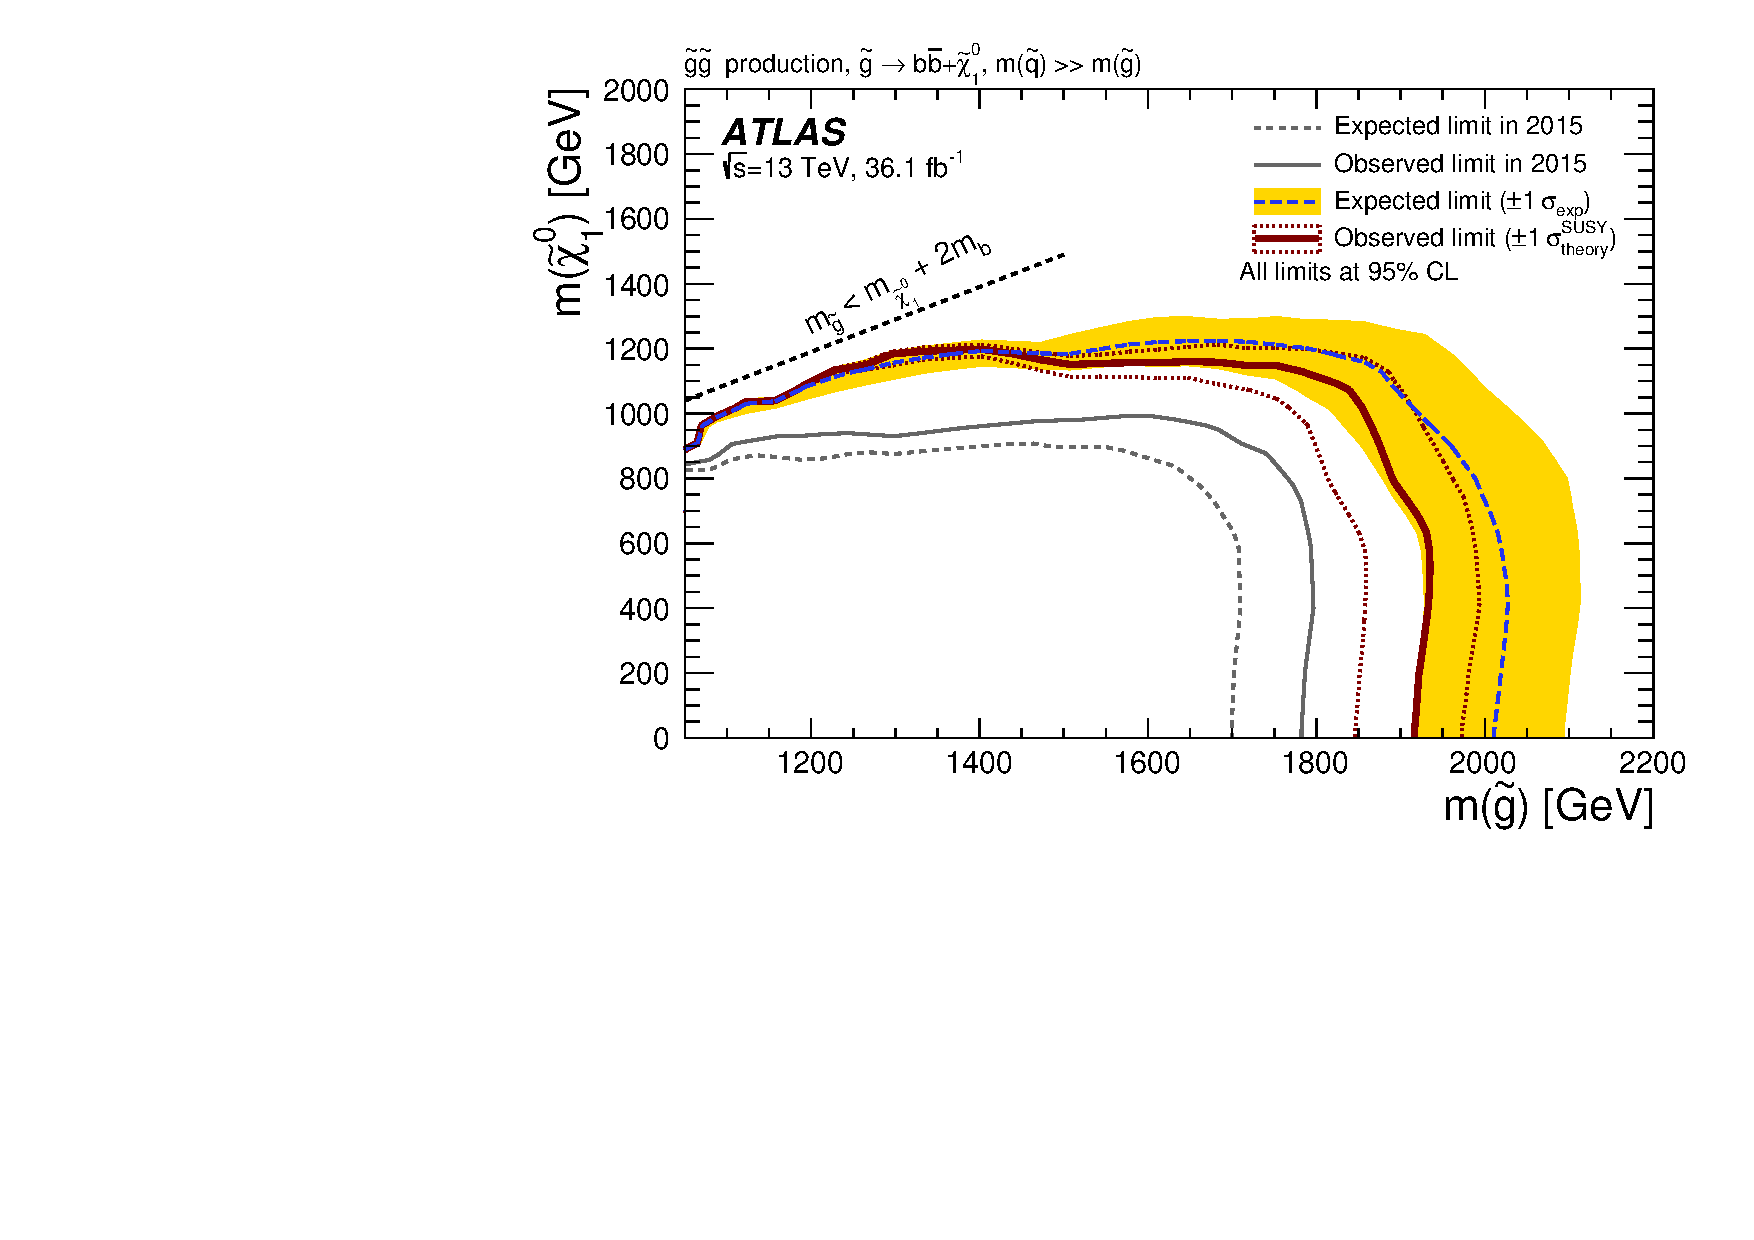
\includegraphics[width=0.75\textwidth]{figures/strong_prod/paper/limits/Limits_Gbb.pdf}\label{fig:limits_Gbb}}
	\caption{Exclusion limits in the $\ninoone$ and $\gluino$ mass plane
  		for the \subref{fig:limits_Gtt} Gtt and  \subref{fig:limits_Gbb} Gbb models obtained
		in the context of the multi-bin analysis. The dashed and solid bold lines
		show the 95\% CL expected and observed limits, respectively. The
  		shaded bands around the expected limits show the
                impact of the
  		experimental and background uncertainties. The dotted
  		lines show the impact on the observed limit of the variation of the
  		nominal signal cross-section by $\pm 1 \sigma$ of its theoretical
  		uncertainty. 
		The 95\%~CL expected and observed limits from the ATLAS search based on 2015 data 
  		\cite{Aad:2016eki} are also shown.}
	\label{fig:limits_GbbGtt}
\end{figure}


\begin{figure}[ht]
	\centering
	\subfigure[]{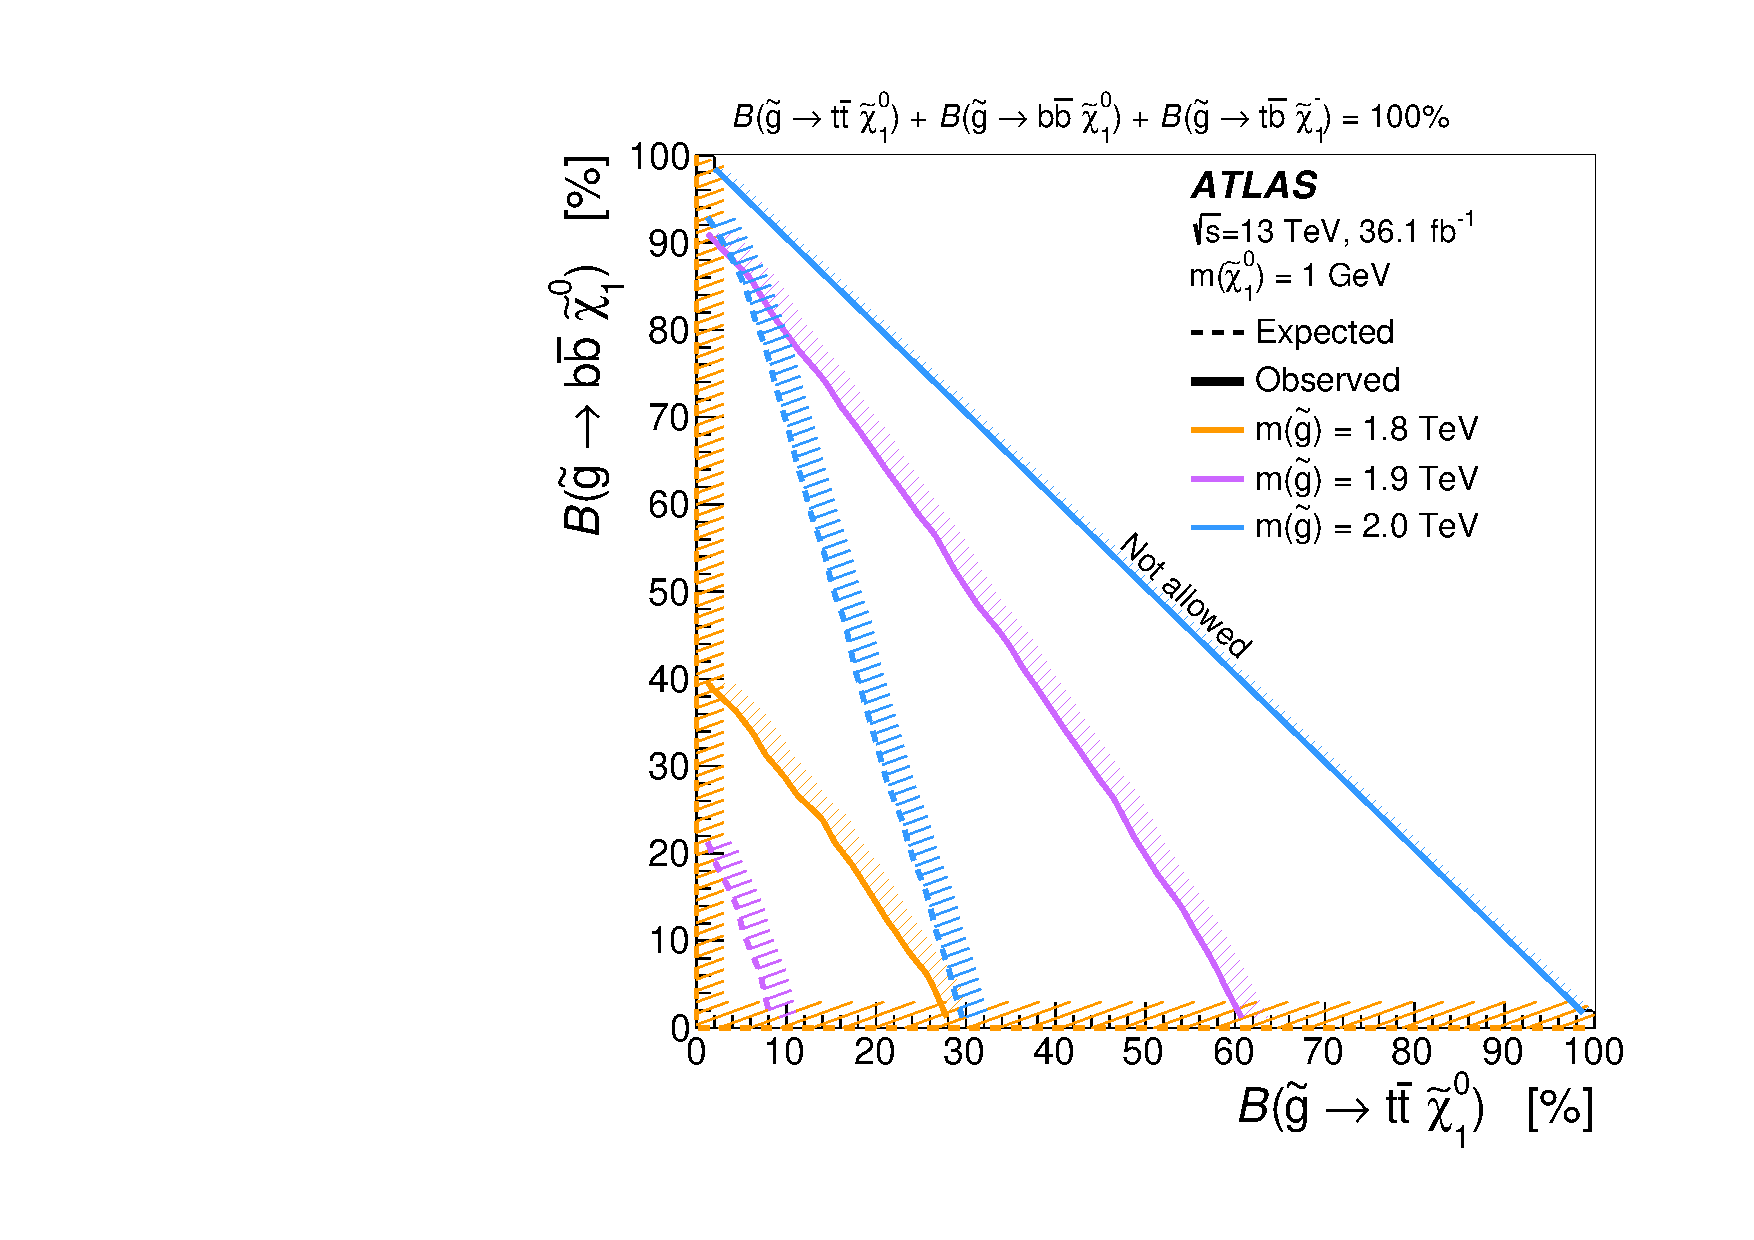
\includegraphics[width=0.63\textwidth]{figures/strong_prod/paper/limits/triangle_UL_massless_neutralino.pdf}\label{fig:limit_br_fixed_neu}}
	\subfigure[]{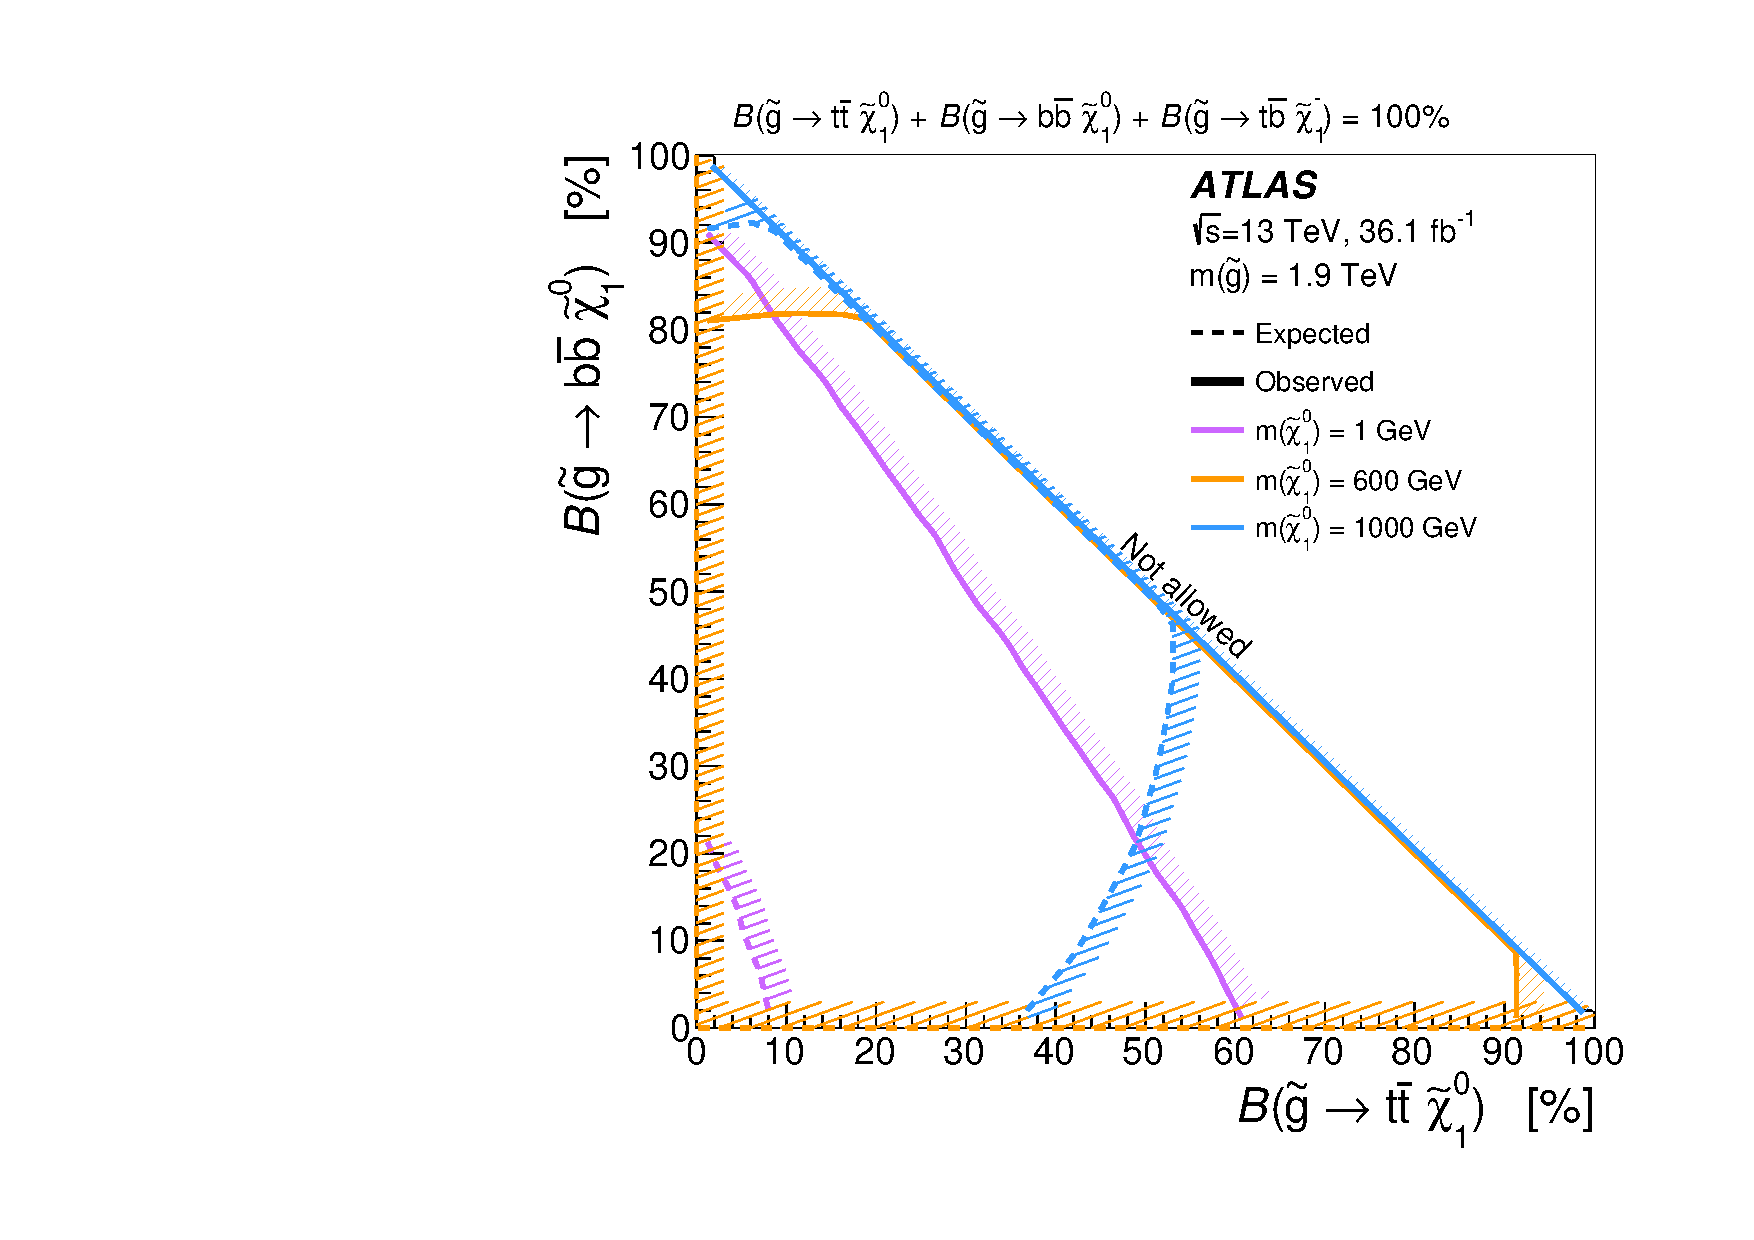
\includegraphics[width=0.63\textwidth]{figures/strong_prod/paper/limits/triangle_UL_1900_gluino.pdf}\label{fig:limit_br_fixed_glu}}
	\caption{Exclusion limits in the $\gluino \to t \bar{t} \ninoone$ and $\gluino \to b \bar{b} \ninoone$
		branching ratio plane assuming \subref{fig:limit_br_fixed_neu} a neutralino mass of 1 GeV and various gluino masses 
		(1.8, 1.9 and 2.0 TeV) and \subref{fig:limit_br_fixed_glu} a gluino mass of 1.9 TeV and three neutralino masses (1, 600 and 1000 GeV). 
		In \subref{fig:limit_br_fixed_neu}, the expected limit for a gluino mass of 1.8 TeV follows the plot axes, meaning that the whole plane is 
		expected to be excluded at 95\% CL.
		The dashed and solid bold lines show the 95\% CL expected and observed limits, respectively. The hashing indicates which side of the line 
		is excluded. The upper right half of the plane is forbidden by the requirement that the sum of branching ratios does not exceed 100\%.}
\end{figure}

\section{Comparison of cut-and-count and multi-bin strategies}

\begin{figure}[ht]
	\centering 
	\subfigure[]{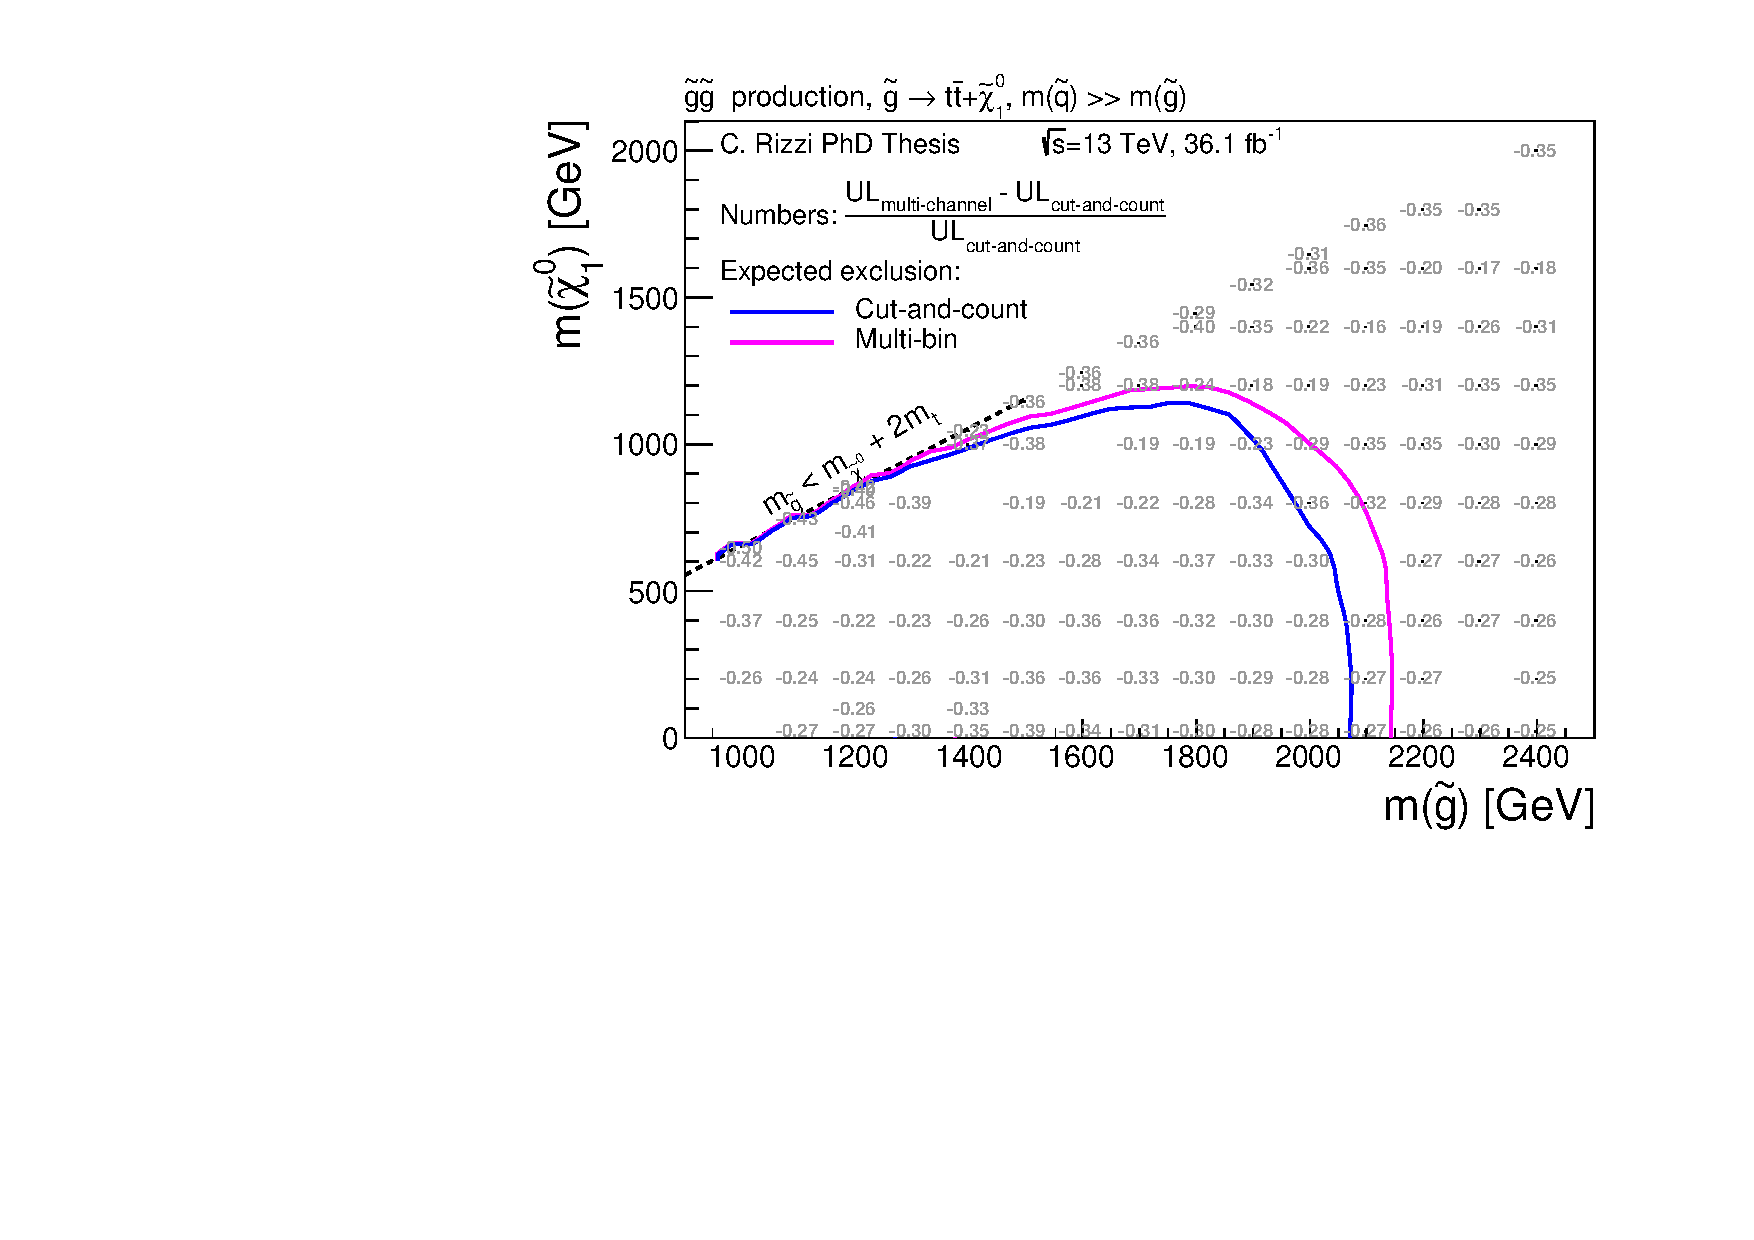
\includegraphics[width=0.75\textwidth]{figures/strong_prod/extra/UL_comp_combi_multich_Gtt.pdf}\label{fig:limits_Gtt_comp}}
	\subfigure[]{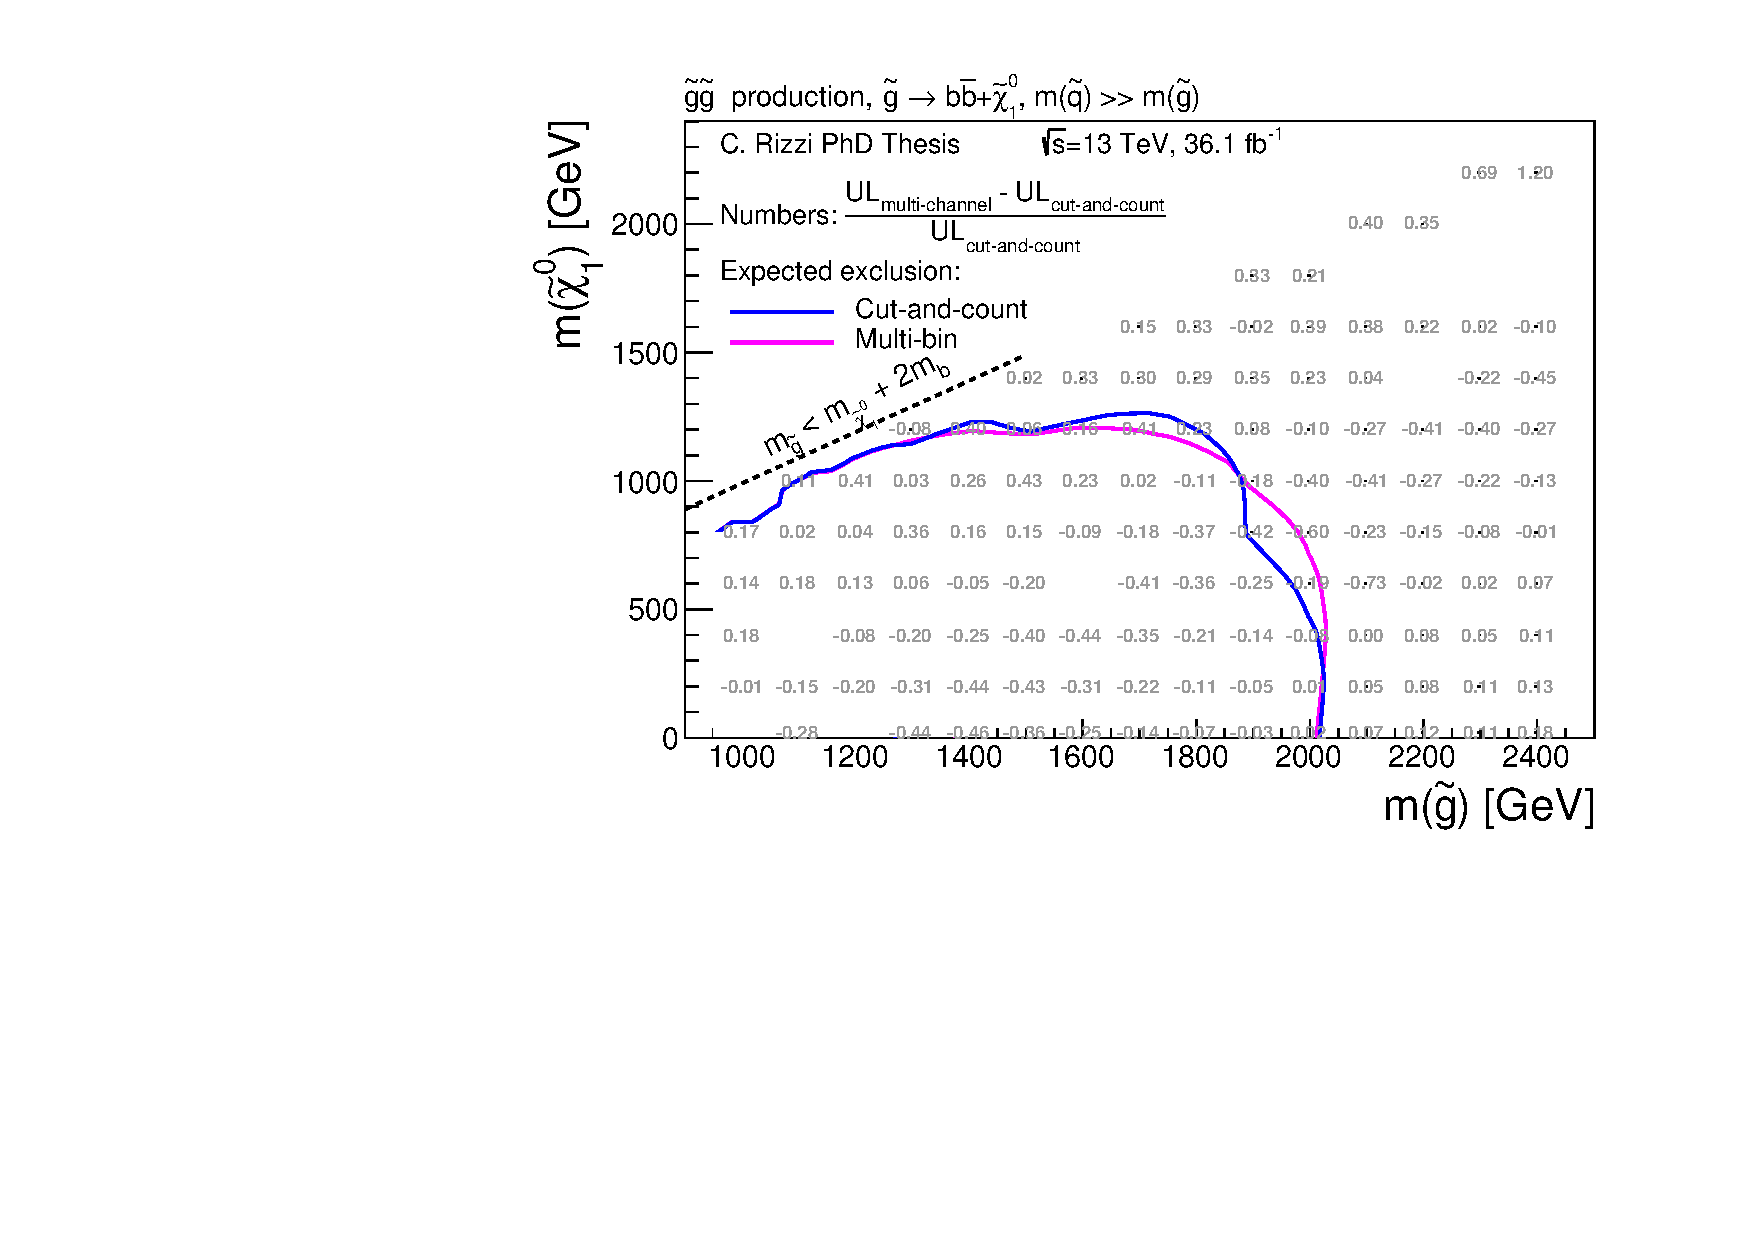
\includegraphics[width=0.75\textwidth]{figures/strong_prod/extra/UL_comp_combi_multich_Gbb.pdf}\label{fig:limits_Gbb_comp}}
	\caption{Exclusion limits in the $\ninoone$ and $\gluino$ mass plane
  		for the \subref{fig:limits_Gtt_comp} Gtt and  \subref{fig:limits_Gbb_comp} Gbb models obtained
		in the context of the multi-bin analysis (pink line) and of the cut-and-count analysis (blue line). 
		The gray numbers show the relative difference in expected \gls{ul} between the multi-bin and the cut-and-count analysis: a negative number shows a lower expected \gls{ul} for the multi-bin analysis.}
	\label{fig:limits_GbbGtt_comp}
\end{figure}

%\section{Results in the context of the ATLAS SUSY group}
